%%%%%%%%%%%%%%%%%%%%%%%%%%%%%%%%%%%%%%%%%%%%%%%%%%%%%%%%%%%%%%%%%%
%%%%%%%% ICML 2014 EXAMPLE LATEX SUBMISSION FILE %%%%%%%%%%%%%%%%%
%%%%%%%%%%%%%%%%%%%%%%%%%%%%%%%%%%%%%%%%%%%%%%%%%%%%%%%%%%%%%%%%%%

% Use the following line _only_ if you're still using LaTeX 2.09.
%\documentstyle[icml2014,epsf,natbib]{article}
% If you rely on Latex2e packages, like most moden people use this:
\documentclass{article}

% use Times
\usepackage{times}
% For figures
\usepackage{xcolor}
\usepackage{graphicx} % more modern
%\usepackage{epsfig} % less modern
\usepackage{subfigure} 

% For citations
\usepackage{natbib}

% For algorithms
\usepackage{algorithm}
\usepackage{algorithmic}

\usepackage{amsmath}
\usepackage{amssymb}
\usepackage{amsthm}

% As of 2011, we use the hyperref package to produce hyperlinks in the
% resulting PDF.  If this breaks your system, please commend out the
% following usepackage line and replace \usepackage{icml2014} with
% \usepackage[nohyperref]{icml2014} above.
\usepackage{hyperref}

% Packages hyperref and algorithmic misbehave sometimes.  We can fix
% this with the following command.
\newcommand{\theHalgorithm}{\arabic{algorithm}}

\newcommand{\YFcomment}[1]{\marginpar{\footnotesize{{\bf YF:} #1}}}
\newcommand{\SCcomment}[1]{\marginpar{\footnotesize{{\bf SC:} #1}}}

\newtheorem{theorem}{Theorem}
\newtheorem{lemma}[theorem]{Lemma}
\newtheorem{collorary}[theorem]{Collorary}

% Employ the following version of the ``usepackage'' statement for
% submitting the draft version of the paper for review.  This will set
% the note in the first column to ``Under review.  Do not distribute.''
\usepackage{icml2014} 
% Employ this version of the ``usepackage'' statement after the paper has
% been accepted, when creating the final version.  This will set the
% note in the first column to ``Proceedings of the...''
%\usepackage[accepted]{icml2014}


% The \icmltitle you define below is probably too long as a header.
% Therefore, a short form for the running title is supplied here:
\icmltitlerunning{Improving the kNN rule for finite training sets}

\begin{document} 

\twocolumn[
\icmltitle{Improving the kNN rule for finite training sets}

% It is OKAY to include author information, even for blind
% submissions: the style file will automatically remove it for you
% unless you've provided the [accepted] option to the icml2014
% package.
\icmlauthor{Sunsern Cheamanunkul}{scheaman@eng.ucsd.edu}
\icmladdress{UCSD,
            9500 Gilman Dr., La Jolla, CA 92093}
\icmlauthor{Yoav Freund}{yfreund@eng.ucsd.edu}
\icmladdress{UCSD,
            9500 Gilman Dr., La Jolla, CA 92093}

% You may provide any keywords that you 
% find helpful for describing your paper; these are used to populate 
% the "keywords" metadata in the PDF but will not be shown in the document
\icmlkeywords{kNN, minimizing KL-divergence, machine learning, ICML}

\vskip 0.3in
]

\begin{abstract}
  Traditionally, the $k$-NN classification rule predicts a label based
  on the majority of the labels in the neighborhood. While it can be
  shown that the majority rule is optimal aymptotically, there is no
  such guarantee for finite training sets. We propose a simple $k$-NN
  rule that incorporates non-majority classes into the prediction. We
  present a number of experiments on both synthetic datasets and
  real-world datasets, including MNIST and SVHN. We show that our new
  rule can achieve lower error rates compared to the majority rule in
  many cases.
\end{abstract} 

\section{Introduction}
\label{sec:intro}

We consider the $k$-nearest neighbor ($k$-NN) classification rule for
multiclass classification problems where the number of classes $m >
2$. Given a set of training examples, the $k$-NN rule predicts the
label of a new example with the majority of the class labels among its
$k$ nearest neighbors. Fix and Hodges~\cite{Fix1951} show that,
asymptotically, the $k$-NN rule achieves the Bayes error rate $r^*$ by
choosing a large enough $k$ but small compared to the number of
examples $n$. Nonetheless, when $n$ is small, there is no guarantee of
how well the $k$-NN algorithm will perform. 

Additionaly, Cover and Hart~\cite{Cover1967} show that, when $k = 1$,
the aymptotic error rate of the $1$-NN rule is upperbounded by $r^*(2
- \frac{m}{m-1}r^*)$. This result suggests that at least a half of the
class information is contained in the nearest neighbor. When the
nearest neighbor does not have all of the class information, it is
possible that the missing class information could be extracted from
other examples in the neighborhood.

In this paper, we propose a modification to the $k$-NN rule which
potentially leverages additional information from the non-majority
class labels in the neighborhood to improve the classification
accuracy. Our approach makes a prediction based on the entire
distribution of the class labels in the neighborhood instead of just
the majority. While the majority rule works well in most cases, it
completely ignores the information from the minority classes which, in
some cases, can contain crucial information.

To motivate our approach, consider the following example. Suppose
there are 3 classes of examples where each class is generated
according to each of the one-dimensional normal distributions depicted in
Figure~\ref{fig:toy_example}. Even though the example $x$ in
Figure~\ref{fig:toy_example} is of class A but it is likely that the
majority of class labels in the neighborhood of $x$ is class B. In
such case, the majority rule will predict class B. However, if we
consider the rest of the examples in the neighborhood of $x$ and we
rarely observe examples from class C, then a better prediction would
have been class A.

\begin{figure}[ht]
\vskip 0.2in
\begin{center}
\centerline{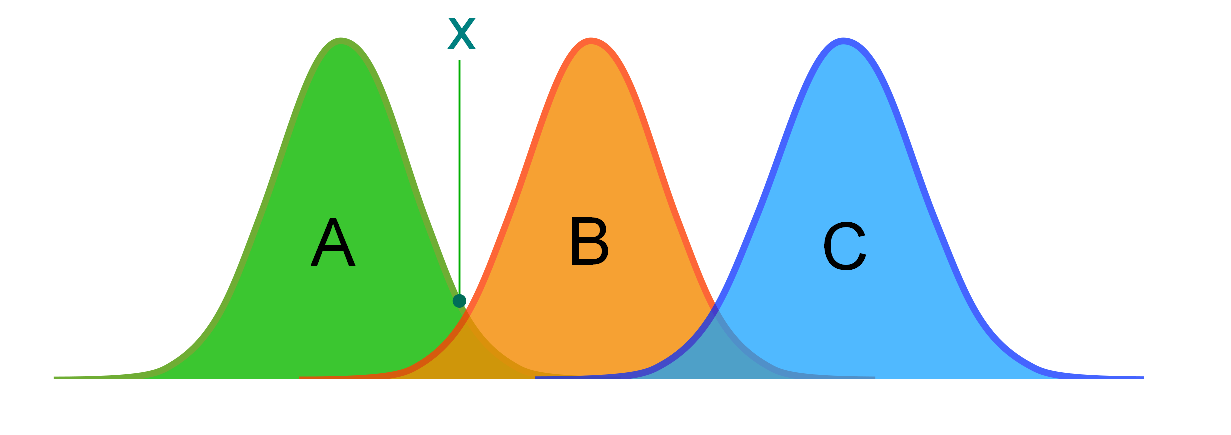
\includegraphics[width=\columnwidth]{figures/toy_example.eps}}
\caption{A toy example showing that the majarity rule (ignoring
  information about class C in the neighborhood) can be
  sub-optimal. Based on the majority rule, the example $x$ of class A
  can be misclassified as class B. However, the rare occurences of
  examples of class C in the neighborhood of $x$ can provide
  useful information regarding the true label of $x$.}
\label{fig:toy_example}
\end{center}
\vskip -0.2in
\end{figure} 

Our approach is related to work on learning label embeddings~
\cite{Collins2009, Bengio2010}. The main difference is that our approach is far
simpler, does not require any convex optimizations and can be
seemlessly integrated into the $k$-NN framework. Another related work
is \cite{Bilmes2001} which introduces a bias term to the likelihood ratio
testing which is justified by the difference between the estimated and
the true class conditional probability.

This paper is organized as follows. In Section~\ref{sec:background},
we describe the framework and the notations. In
Section~\ref{sec:min_kl}, we describe our approach and
justification. In Section~\ref{sec:results}, we present experiments
comparing our approach with the traditional $k$-NN algorithm using
both synthetic data and real-world data. Then, we discuss the results
in Section~\ref{sec:discussion} and conclude the paper in
Section~\ref{sec:conclusion}.

\section{Background}
\label{sec:background}

\newcommand{\X}{\mathcal{X}}
\newcommand{\Y}{\mathcal{Y}}
\newcommand{\trainset}{\mathcal{S}}

Let $\trainset = \{ (x_1,y_1,) \ldots (x_N,y_N)\}$ be a set of
training examples where each instance $x_i$ comes from an example
space $\X$ of which the distance between any two examples is measured
by $d(\cdot,\cdot)$. Without loss of generality, we assume that each
label $y_i$ takes on a value from $\Y = \{1,2,\ldots,m\}$. To simplify
the analysis, we assume that the distribution of classes is uniform
and the number of examples per class is denoted by $n$.

\newcommand{\nh}{\mathcal{N}}
\newcommand{\Pemp}{\widehat{\mathbf{P}}_{(x,\trainset,k)}}
\newcommand{\Ptrue}{\mathbf{P}_{(x)}}

Let $\nh_k(x)$ denote the neighborhood of size $k$ of an example $x
\in \X$ with respect to the distance measure $d$. The traditional
$k$-NN rule predicts the label of an example $x$ with the majority of
the labels in $\nh_k(x)$. More formally, given $x$ and $\nh_k(x)$, we
can define an empirical distribution $\Pemp$ such that, for each $i \in \Y$, 
\[
\Pemp(i) = \frac{\#\{ \mbox{occurrences of label } i \mbox{ in } \nh_k(x)\}}{k}
\]
The $k$-NN rule predicts the label $\hat{y}$ such that
\[
\hat{y} = \arg\max_{i \in \Y} \: \Pemp(i)
\]

For any example $x \in \X$, we can consider the true class
distribution of $x$, denoted by $\Ptrue$ which is given by, for each $i \in \Y$,
\[
\Ptrue(i) = \Pr(Y=i | X=x)
\]
Under certain assumptions, it is shown in \cite{Fix1951} that,
for every class label $i \in \Y$, 
\[
\lim_{\substack{n \to \infty\\k \to \infty\\k/n \to 0}} \Pemp(i) = \Ptrue(i)
\]
Therefore, the majority rule is asymptotically optimal. However, in
the finite sample scenario, it can be sub-optimal due to the discrepancy
between the empirical distribution $\Pemp$ and the true distribution
$\Ptrue$ as demonstrated by the toy example in
Figure~\ref{fig:toy_example}.

\section{Minimizing KL-Divergence Rule}
\label{sec:min_kl}

\newcommand{\dkl}{D_{\mathrm{KL}}}
\newcommand{\Qemp}{\widehat{\mathbf{Q}}_{(j,\trainset,k)}}

We propose a new $k$-NN rule that predicts the class label based on
the entire class distribution $\Pemp$ instead of just the mode
(majority) of $\Pemp$. We refer to this rule as the minimizing
KL-divergence rule (MinKL). Given a training set $\trainset$ and the
neighborhood of size $k$, we define, for each class $j$, an empirical
center distribution $\Qemp$ as
\[
\Qemp = \frac{\sum_{(x,j) \in \trainset_j} \Pemp}{|\trainset_j|}
\]
where $\trainset_j = \{ (x,y) \in \trainset | y = j \}$ consists of
all examples with class label $j$.  To classify a new example $x$, the
empirical class distribution $\Pemp$ is compared to each of the center
distributions $\Qemp$ with respect to the KL-divergence $\dkl(\Pemp ||
\Qemp)$ and the class label that minimizes the distance is then
predicted. More formally, the predicted label $\hat{y}$ is given by
\[
\hat{y} = \arg\min_{j \in \Y} \: \dkl(\Pemp || \Qemp) 
\]
where the KL-divergence between two discrete distributions
$\mathbf{p}$ and $\mathbf{q}$ is defined as
\[
\dkl(\mathbf{p} || \mathbf{q}) = \sum_i \mathbf{p}(i) \log
\frac{\mathbf{p}(i)}{\mathbf{q}(i)}
\]

A summary of the algorithm is given in
Algorithm~\ref{alg:minkl_training} and
Algorithm~\ref{alg:minkl_predict}.

\newcommand{\Q}{\mathbf{Q}}

\begin{algorithm}[tb]
\caption{The MinKL $k$-NN rule: Training}
\label{alg:minkl_training}
\begin{algorithmic}[1]
\REQUIRE{Training set $\trainset$ and $k$}
\OUTPUT{The center distributions $\widehat{\Q}_j$ for all $j \in \Y$}
\STATE $\widehat{\Q}_j \leftarrow \vec{0} \mbox{ for } j \in \Y$
\FOR{each example $(x,j) \in \trainset$}
\STATE $\widehat{\Q}_j \leftarrow \widehat{\Q}_j + \Pemp$
\ENDFOR
\STATE $\widehat{\Q}_j \leftarrow \widehat{\Q}_j / |\trainset_i|
\mbox{ for all } j \in \Y$
\end{algorithmic}
\end{algorithm}

\begin{algorithm}[tb]
\caption{The MinKL $k$-NN rule: Prediction}
\label{alg:minkl_predict}
\begin{algorithmic}[1]
  \REQUIRE{Training set $\trainset$,\\
    A test example $x$,\\
    The center distributions $\widehat{\Q}_j$ for all $j \in \Y$ } 
  \OUTPUT{Predicted label $\hat{y}$} 
  \STATE $\hat{y} = \arg\min_{i \in \Y} \dkl(\Pemp || \widehat{\Q}_i)$
\end{algorithmic}
\end{algorithm}

\newcommand{\Pexpected}{\overrightarrow{\mathbf{P}}_{(x,k)}}
\newcommand{\Qexpected}{\overrightarrow{\mathbf{Q}}_{(j,k)}}

To analyze our approach in the finite sample setup, we introduce a few
more notations. Let $\Pexpected$ denote the expected class
distribution of an example $x$ induced by a neighborhood of size $k$,
which is given by
\[
\Pexpected = \mathbf{E}_{\trainset}[\Pemp]
\]
Similarly, let $\Qexpected$ denote the expected center distribution
for examples of class $j$ defined by
\[
\Qexpected =\mathbf{E}_{\trainset}[\Qemp]
\]
Note that the expectation is taken over all possible training sets of
size $N$.

Ideally, the empirical distribution $\Pemp$ should be compared to the
expected center distribution $\Qexpected$. However, in practice, we
use $\Qemp$ as an estimate for $\Qexpected$. This is reasonable
because $\Qemp$ for each class $j$ is estimated from a relatively
large amount of examples in the training set.

For any training set $\trainset$ and for any $k$, there exists some
$\delta_k > 0$ such that
\[
\dkl(\Pexpected || \Qemp) < \delta_k \; \forall \; (x,j) \in \trainset
\]

When $\delta_k = 0$, our algorithm can be justified by a direct
application of Lemma~\ref{lemma:dkl} and Collorary~\ref{col:min_dkl}.

\newcommand{\sampleYK}{y^k}
\newcommand{\sampleEmpDist}{\mathbf{P}_{y^k}}

Let $\sampleYK = [y_1, \ldots, y_k]$ denote a sample of size $k$ drawn IID
from a fixed distribution over $Y$ and let $\sampleEmpDist$ denote the
empirical distribution induced by the sample
$\sampleYK$. Specifically,
\[
\sampleEmpDist(i) = \frac{\#\{ \mbox{occurrences of } i \mbox{ in } y^k\}}{k}
\]

\begin{lemma}
\label{lemma:dkl}
For any distribution $\Q$ and for any sample $\sampleYK$, the
likelihood of $\sampleYK$ drawn from $\Q$ is given by
\[
\Q(y^k) = 2^{-k(H(\sampleEmpDist) + \dkl\sampleEmpDist || \Q))}
\]
\end{lemma}
\begin{proof}
  \begin{align*}
    \Q(y^k) 
&= \prod_{l=1}^k \Q(y_l)\\ 
&= \prod_{j \in \Y} Q(j)^{n\sampleEmpDist(j)}\\ 
&= \prod_{j \in \Y} 2^{n\sampleEmpDist(j) \log \Q(j)}\\ 
&= \prod_{j \in \Y} 2^{n(\sampleEmpDist(j) \log \Q(j) - \sampleEmpDist(j) \log \sampleEmpDist(j) + \sampleEmpDist(j) \log \sampleEmpDist(j))}\\ 
&= 2^{k \sum_{j \in \Y} (-\sampleEmpDist(j) \log \frac{\sampleEmpDist(j)}{\Q(j)} + \sampleEmpDist(j) \log \sampleEmpDist(j))}\\ 
&= 2^{k(-\dkl(\sampleEmpDist||\Q) - H(\sampleEmpDist))}\\
  \end{align*}
\end{proof}

\begin{collorary}
\label{col:min_dkl}
Given a set of distributions $\mathcal{Q} = \{\Q_1,\Q_2, \ldots,
\Q_{m}\}$ and a sample $\sampleYK$ drawn from any distribution, the
likelihood of $\sampleYK$ is maximized under $\Q_{i^*}$ if and only if
the KL-divergence from $\sampleEmpDist$ to $\Q_{i^*}$ is minimized.
\[
 i^* = \arg\max_{i \in \Y} \log \Q_i(y^k) = \arg\min_{i \in \Y} \dkl(\sampleEmpDist||\Q_i)
\]
\end{collorary}
\begin{proof}
  Applying Lemma~\ref{lemma:dkl}, we have
  \begin{align*}
    \Q_i(y^k) &= 2^{-n(H(\sampleEmpDist) + \dkl\sampleEmpDist || \Q_i))}\\
    \log \Q_(y^k) &= -n(H(\sampleEmpDist) + \dkl(\sampleEmpDist || \Q_i))\\
    \arg\max_{i \in \Y} \log \Q(y^k) &= \arg\max_{i \in \Y} - n\dkl(\sampleEmpDist || \Q_i))\\ 
    &= \arg\min_{i \in \Y} \dkl(\sampleEmpDist || \Q_i))\\
  \end{align*}
\end{proof}

\newcommand{\Qempjstar}{\widehat{\mathbf{Q}}_{(j^*,\trainset,k)}}

\iffalse
However, when $\delta_k > 0$, we need to enforce a stronger assumption
about the data in the training set in order to justify our
algorithm. Suppose $j^*$ is the true class for an example
$x$. Intuitively, our approach will be justified if the expected
center distributions $\Qexpected$ for incorrect classes are far enough
from the empirical distribution $\Pemp$. Specifically, suppose
\begin{small}
\[
\dkl(\Pemp || \Pexpected) \le \dkl(\Pemp || \Qexpected) + \delta_k
\; \forall j \ne j^*
\]
\end{small}
We can then justify our approach using information geometry. For any
$\delta_k > 0$, we have
\[
\dkl(\Pemp || \Pexpected) \le \dkl(\Pemp || \Qempjstar) + \delta_k
\]
Hence, it follows that 
\begin{small}
\[
\dkl(\Pemp || \Qempjstar) \le \dkl(\Pexpected || \Qemp) \; \forall  j \ne j^*
\]
\end{small}
\fi

It is worth noting that our algorithm will reduce to the majority
rule when the prototypical distribution
$\Qemp$ is defined as 
\[
\Qemp(i) = \begin{cases} 1-\epsilon &\mbox{if } i = j \\ 
\epsilon & \mbox{otherwise} \end{cases}
\]
where $\epsilon$ is a small constant. In this case, the non-majority
examples do not contribution any information to the final
prediction. Hence, the prediction will be made based solely on the
majority.

\section{Experiments}
\label{sec:results}
In this section, we describe experiments we have performed with both
synthetic data and real-world data. For each dataset, we compare the
error rates of the $k$-NN with the minimizing KL-divergence rule
(MinKL) to those of the $k$-NN with the majority rule (Majority) under
various conditions. A summary of the datasets is given in
Table~\ref{table:results}.

\begin{table}[tb]
\caption{A summary of the datasets.}
\label{table:results}
\vskip 0.1in
\begin{center}
\begin{scriptsize}
\begin{sc}
\begin{tabular}{lcccc}
  \hline
  \abovespace\belowspace
  Dataset & No. of classes & No. of train ex. & No. of test ex. \\
  \hline
  \abovespace
  SYN-1 & 10 & up to 1600 & 10000\\
  SYN-2 & 64 & up to 6400 & 6400\\
  \belowspace
  SYN-3 & 10 & up to 1600 & 10000\\
  \hline
  \abovespace
  uRight & 26 & 9945 & -  \\
  MNIST & 10 & 60000 & 10000 \\
  \belowspace
  SVHN & 10 & 73257 & 26032\\
  \hline
\end{tabular}
\end{sc}
\end{scriptsize}
\end{center}
\vskip -0.1in
\end{table}

\subsection{Synthetic data}
We performed 3 experiments using synthetic data that can be described
as follows. Each example $x$ is a point inside a wrap-around
$d$-dimensional hypercube of size $b$, or $x \in [0,b-1]^d$. The
instances of each class are generated by a normal distribution with
mean located at each integer lattice point of the hypercube and a
covariance matrix $\sigma \mathbf{I}_d$. Thus, the total number of
classes is $b^d$. The distribution of the classes in each dataset is
uniform. In Figure~\ref{fig:synthetic}, the generating distributions
of each dataset are shown in the left-most column. The Manhattan
distance ($L_1$ norm) is used for measuring the distance between
examples.

In our first experiment, we generated a dataset called \textbf{SYN-1}
using the following parameters: $b=10, d=1$ and
$\sigma=1.5$. \textbf{SYN-1} was intended to mimic the situation
described in Figure~\ref{fig:toy_example}. The number of classes in
\textbf{SYN-1} is 10. In the second experiment, we generated another
dataset called \textbf{SYN-2} using the following parameters: $b=4$,
$d=3$ and $\sigma=0.4$. \textbf{SYN-2} has a very similar structure to
\textbf{SYN-1} but it is more complex with the total of $64$
classes. In our third experiment, we generated yet another dataset
called \textbf{SYN-3}. Similar to \textbf{SYN-1}, each instance of
\textbf{SYN-3} is one-dimensional. However, the generating
distribution for class $i$ is a mixture of two normal distributions
centered at $i$ and $i+3$ and the mixing coefficient is 0.8 and 0.2
respectively. \textbf{SYN-3} is intended for simulating when
$\delta_k > 0$.  

In Figure~\ref{fig:synthetic}, we compare the error rates of MinKL and
Majority using different $n$ and $k$ for each dataset. For each $n$,
we ran both MinKL and Majority for $k$ ranged. The center column of
Figure~\ref{fig:synthetic} shows the error rates for different $k$
when $n$ is fixed at 20 per classes for each dataset. Then, for each
$n$, the best error rate of both MinKL and Majority over $k$ are shown
in the right-most column of Figure~\ref{fig:synthetic}. The error
rates of both MinKL and Majority converge to the Bayes error as $n$
increases. In \textbf{SYN-1} and \textbf{SYN-2}, MinKL converges
faster than Majority and is able to attain lower error rates
especially when $n$ is small. However, in \textbf{SYN-3}, MinKL has
higher average error rates than Majority for when $n$ is small.

\begin{figure*}[tb]
\vskip 0.2in
\begin{center}
\centering
\subfigure[SYN-1: (left) Data models, (center) error rate vs. $k$
while $n$ fixed, (right) error rate vs. $n$ while $k$ fixed]{
  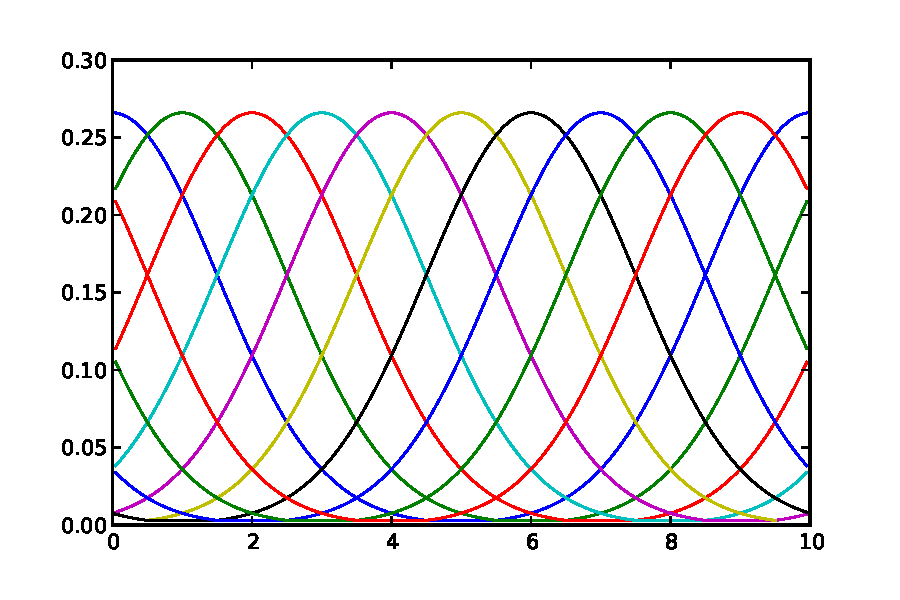
\includegraphics[width=.33\linewidth]{figures/icml-syn1-data.pdf}
  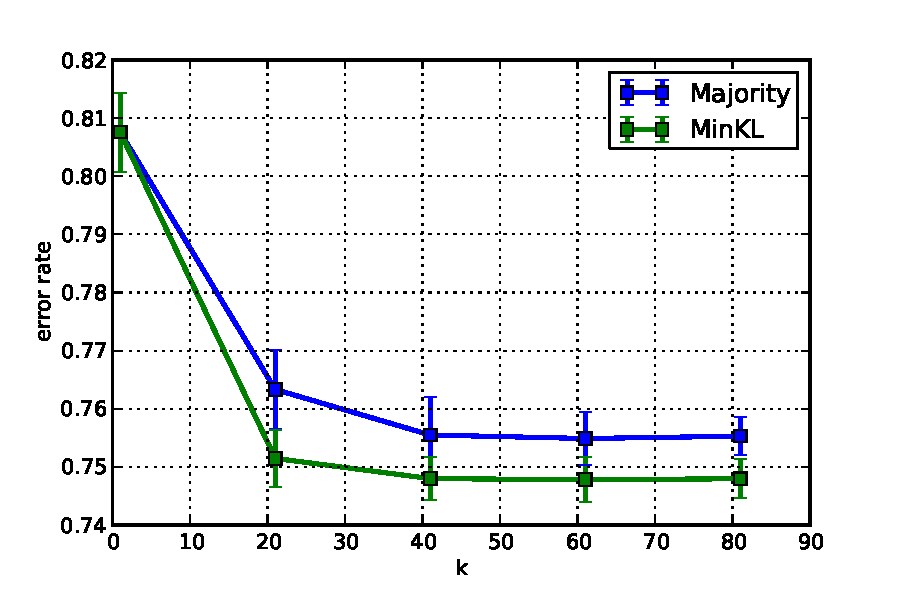
\includegraphics[width=.33\linewidth]{figures/icml-syn1-results-N20.pdf}
  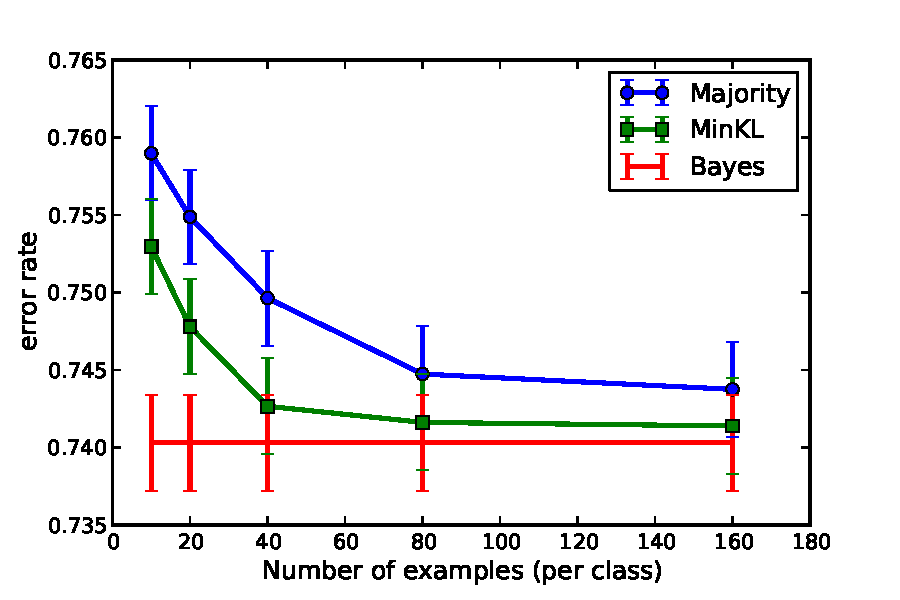
\includegraphics[width=.33\linewidth]{figures/icml-syn1-overall.pdf}
  \label{fig:synthetic-1}
}\\
\subfigure[SYN-2: (left) Data models, (center) error rate vs. $k$
while $n$ fixed, (right) error rate vs. $n$ while $k$ fixed]{
  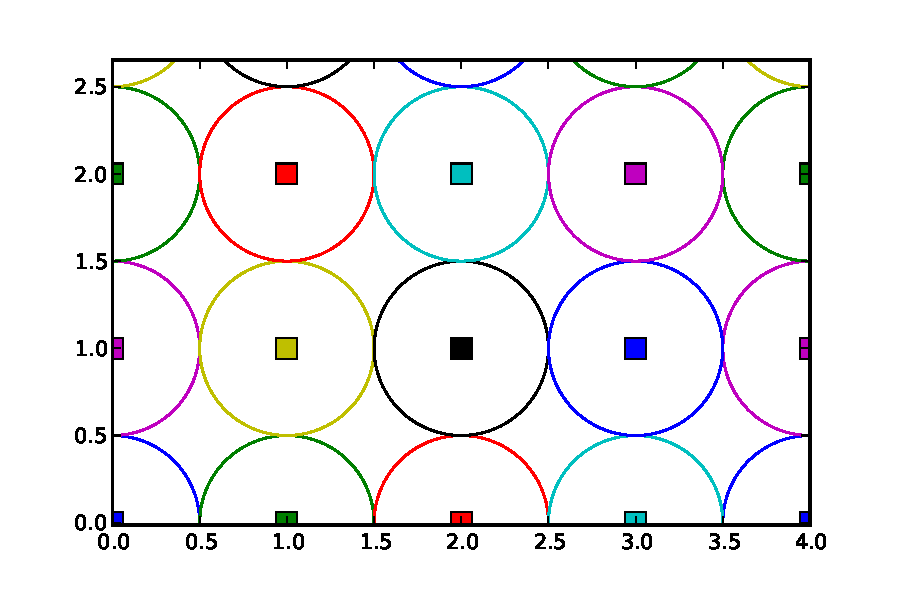
\includegraphics[width=.33\linewidth]{figures/icml-syn2-data.pdf}
  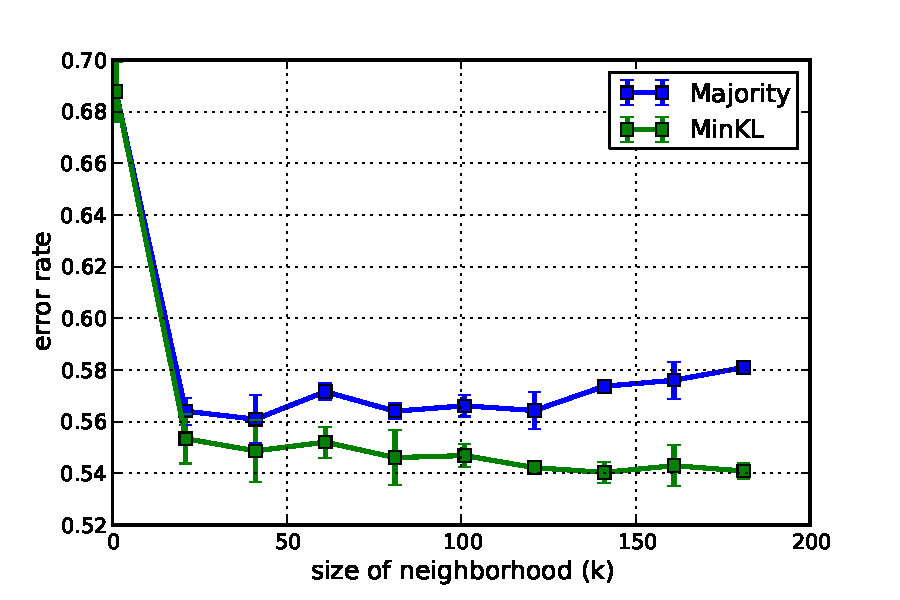
\includegraphics[width=.33\linewidth]{figures/icml-syn2-results-N20.pdf}
  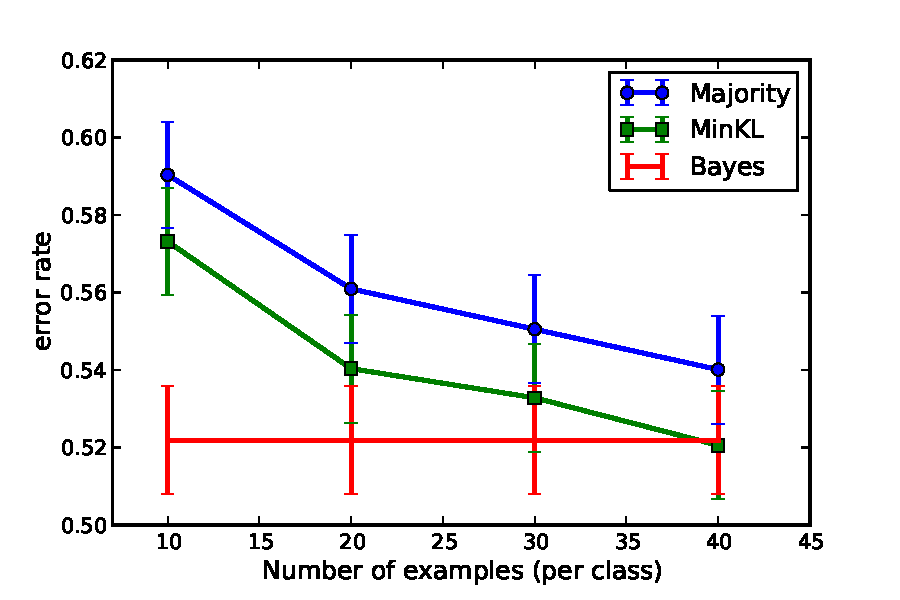
\includegraphics[width=.33\linewidth]{figures/icml-syn2-overall.pdf}
  \label{fig:synthetic-2}
}\\
\subfigure[SYN-3: (left) Data models, (center) error rate vs. $k$
while $n$ fixed, (right) error rate vs. $n$ while $k$ fixed]{
  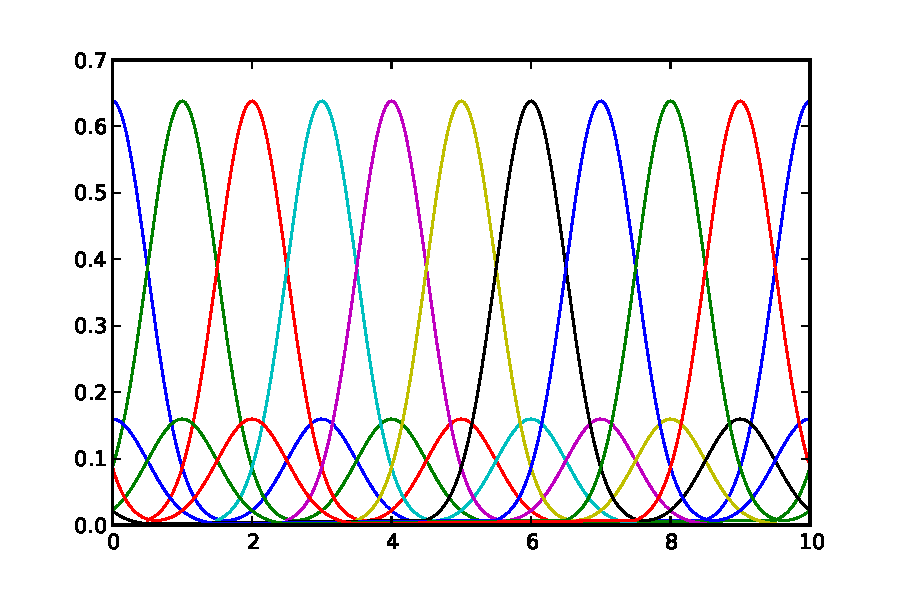
\includegraphics[width=.33\linewidth]{figures/icml-syn3-data.pdf}
  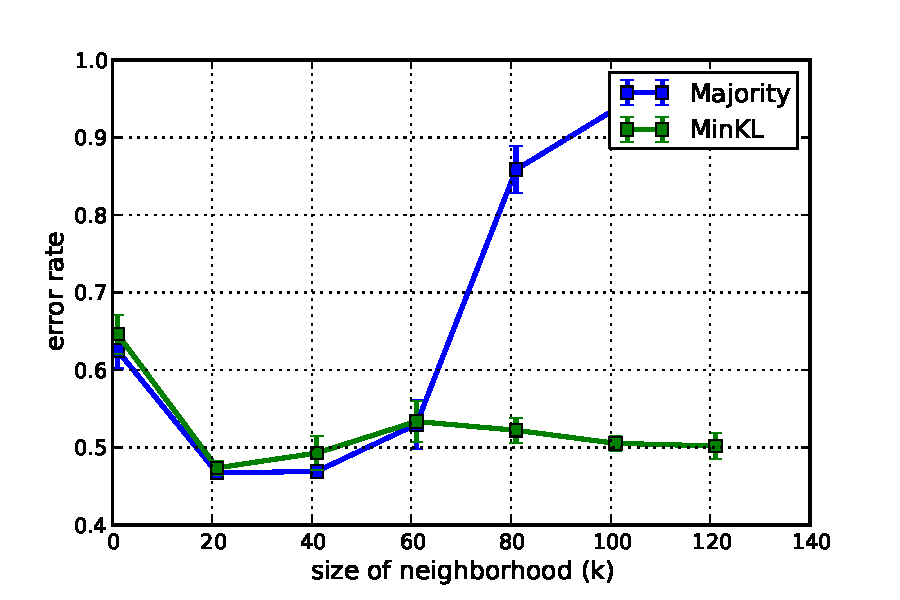
\includegraphics[width=.33\linewidth]{figures/icml-syn3-results-N20.pdf}
  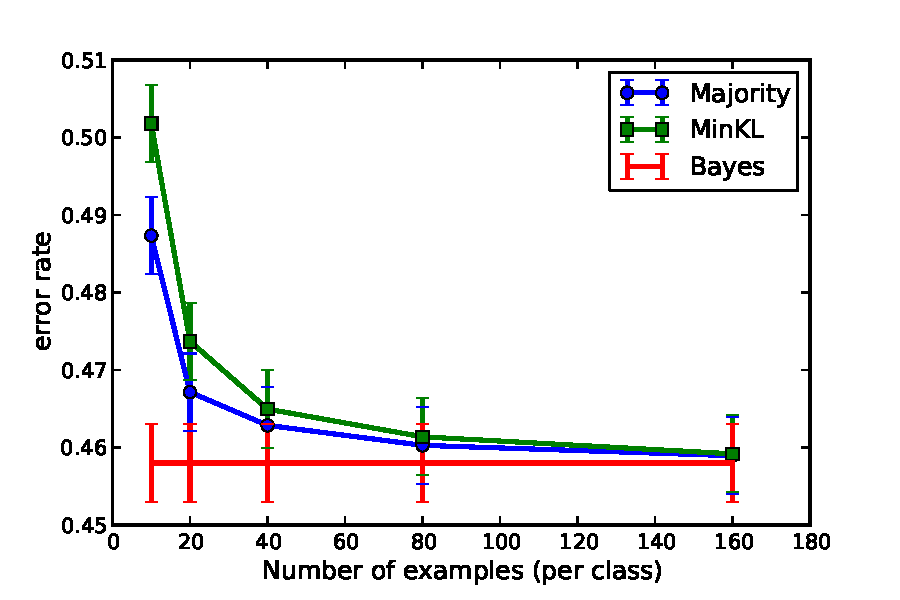
\includegraphics[width=.33\linewidth]{figures/icml-syn3-overall.pdf}
  \label{fig:synthetic-3}
}
\caption{Results from the synthetic data experiment.}
\label{fig:synthetic}
\end{center}
\vskip -0.2in
\end{figure*}

\subsection{uRight}
The uRight dataset contains handwriting trajectories of the 26
lowercase English characters.  We collected the handwriting data from
15 different users writing isolated lowercase English characters on a
touch screen of a mobile phone with their fingers. Each example is a
sequence of $(x,y,t)$ where $x$ and $y$ are the $(x,y)$-coordinates
and $t$ is the timestamp of each sample
point. Figure~\ref{fig:uright-examples} shows some examples of the
handwriting trajectories. There are 9945 examples in the dataset and
the distribution of the class labels is fairly uniform. The similarity
between two examples is measured by the dynamic time wraping (DTW)
distance~\cite{Bahlmann2004}.

Using $k = 5$, the average error rates of MinKL and Majority for each
user are summarized in Figure~\ref{fig:uright-results}. According to
the paired t-test, the average error rate of MinKL (3.76\%) is
significantly smaller than the average error rate of Majority (5.86\%)
with $p$-value $ < 0.001$. Figure~\ref{fig:uright-mistakes} displays
some of the examples that were misclassified by Majority but correctly
classified by MinKL.

\begin{figure}[htb]
\vskip 0.2in
\begin{center}
\centering
  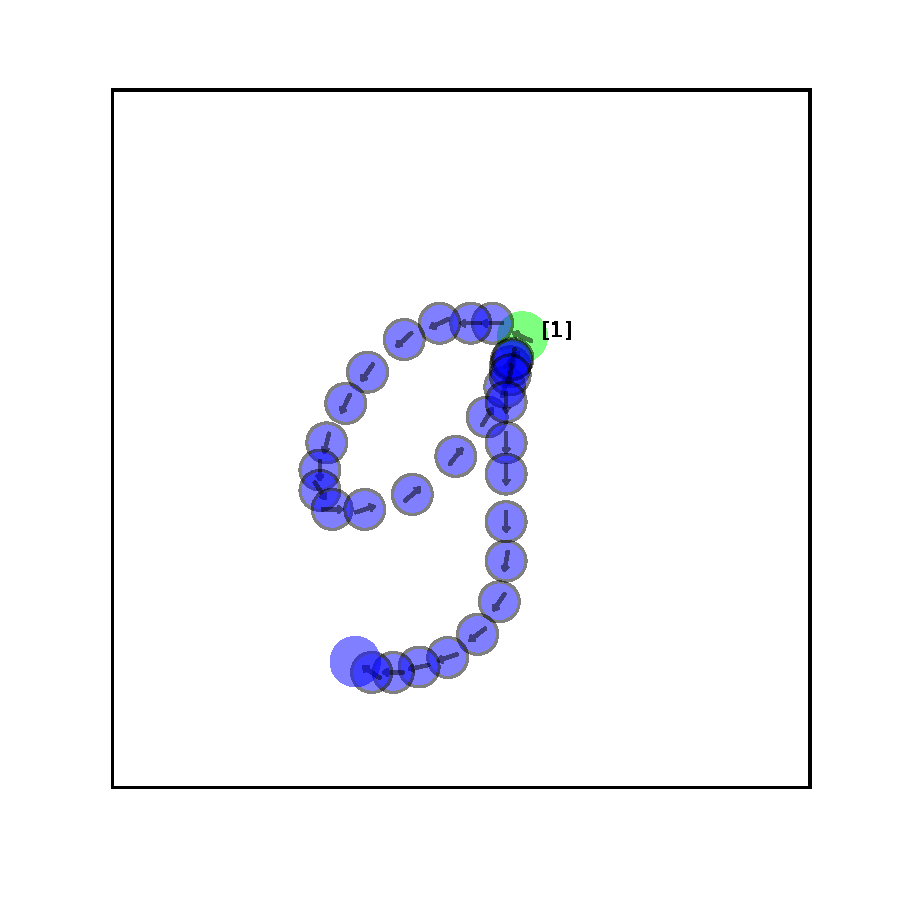
\includegraphics[width=.3\linewidth]{figures/icml-uright-examples-0.pdf}
  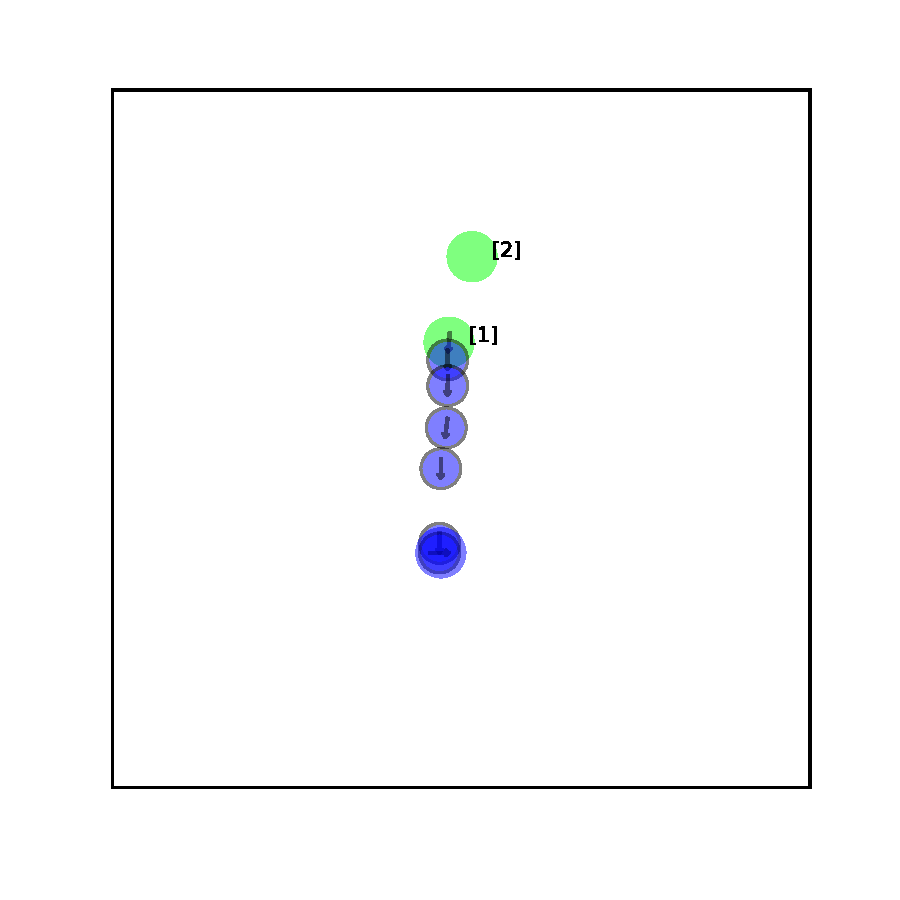
\includegraphics[width=.3\linewidth]{figures/icml-uright-examples-1.pdf}
  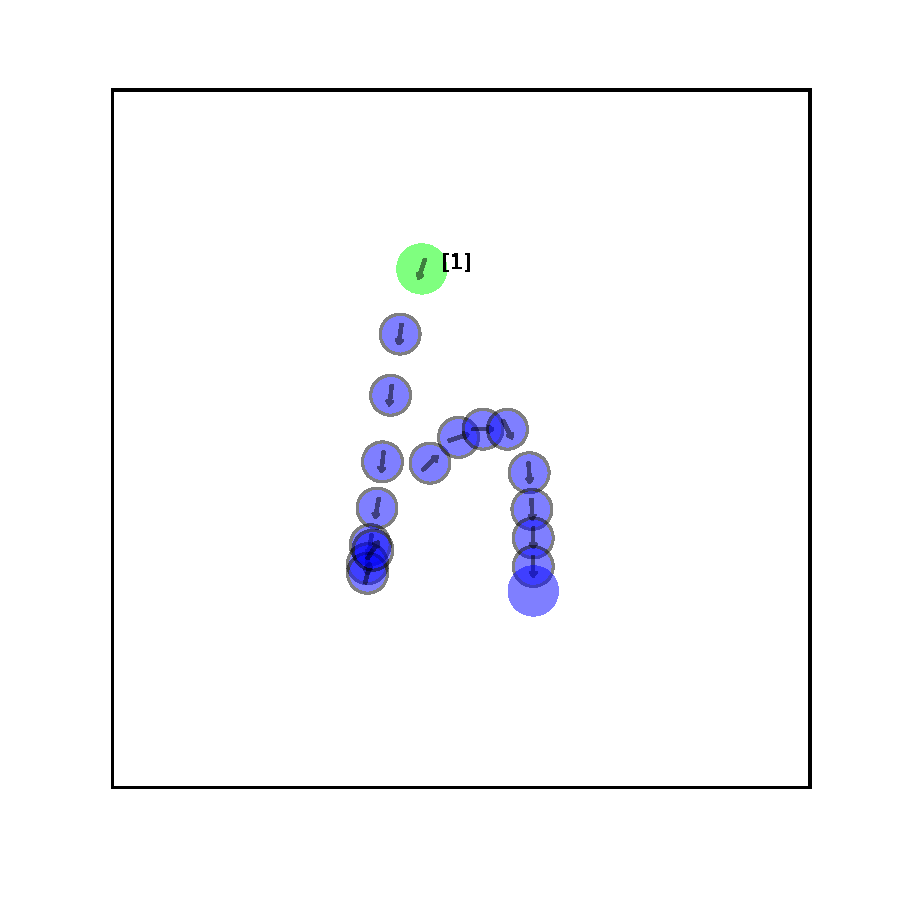
\includegraphics[width=.3\linewidth]{figures/icml-uright-examples-2.pdf}\\
  %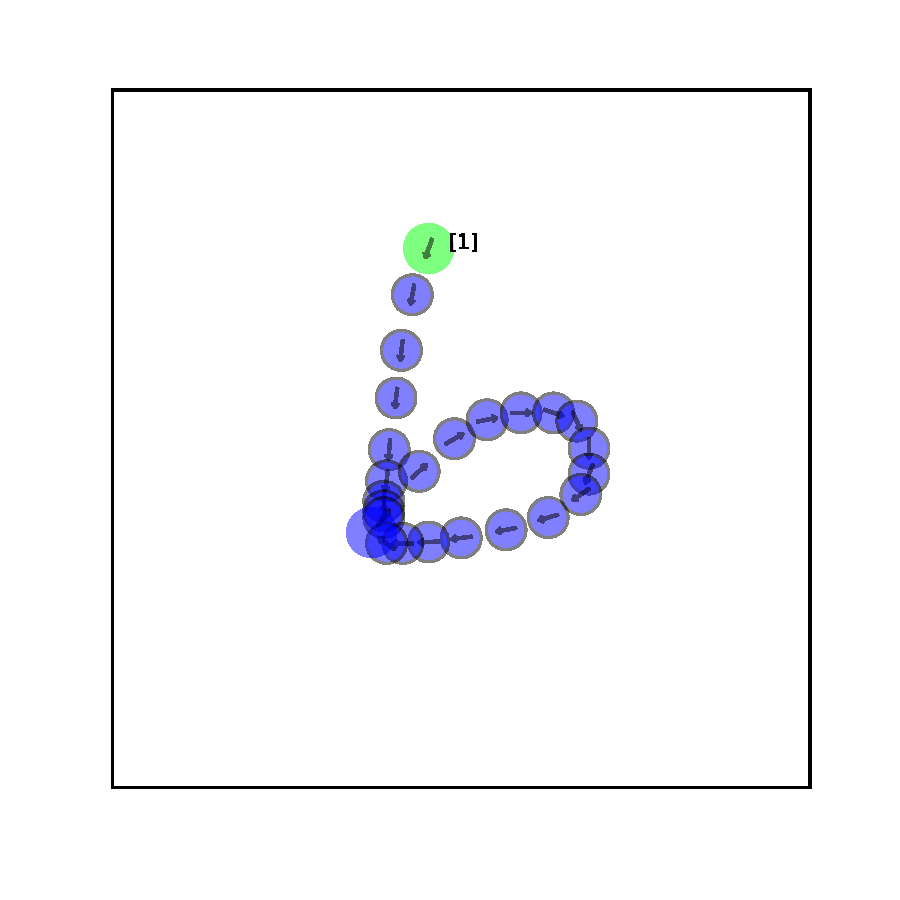
\includegraphics[width=.3\linewidth]{figures/icml-uright-examples-3.pdf}
  \caption{Some examples from the uRight handwriting dataset.}
  \label{fig:uright-examples}
\end{center}
\vskip -0.2in
\end{figure}

\begin{figure}[htb]
\vskip 0.2in
\begin{center}
\centering
  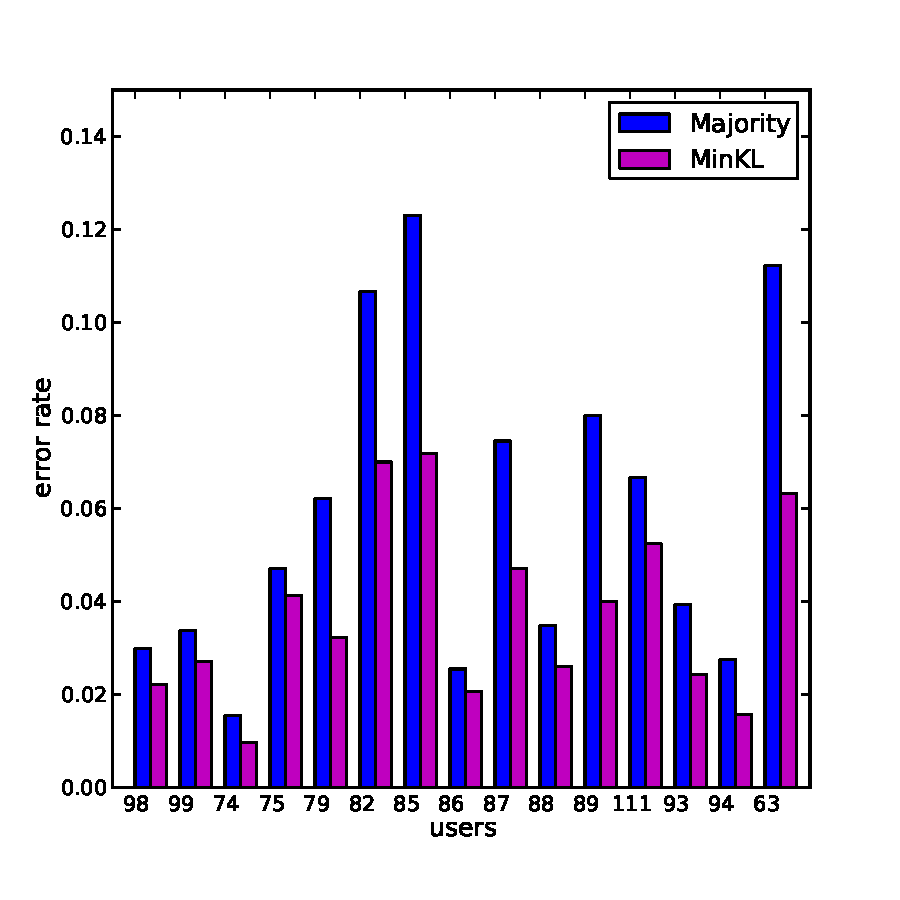
\includegraphics[width=.95\linewidth]{figures/icml-uright-allusers.pdf}
  \caption{The average error rates of MinKL and Majority for each user.}
  \label{fig:uright-results}
\end{center}
\vskip -0.2in
\end{figure}

\begin{figure}[htb]
\vskip 0.2in
\begin{center}
\centering
  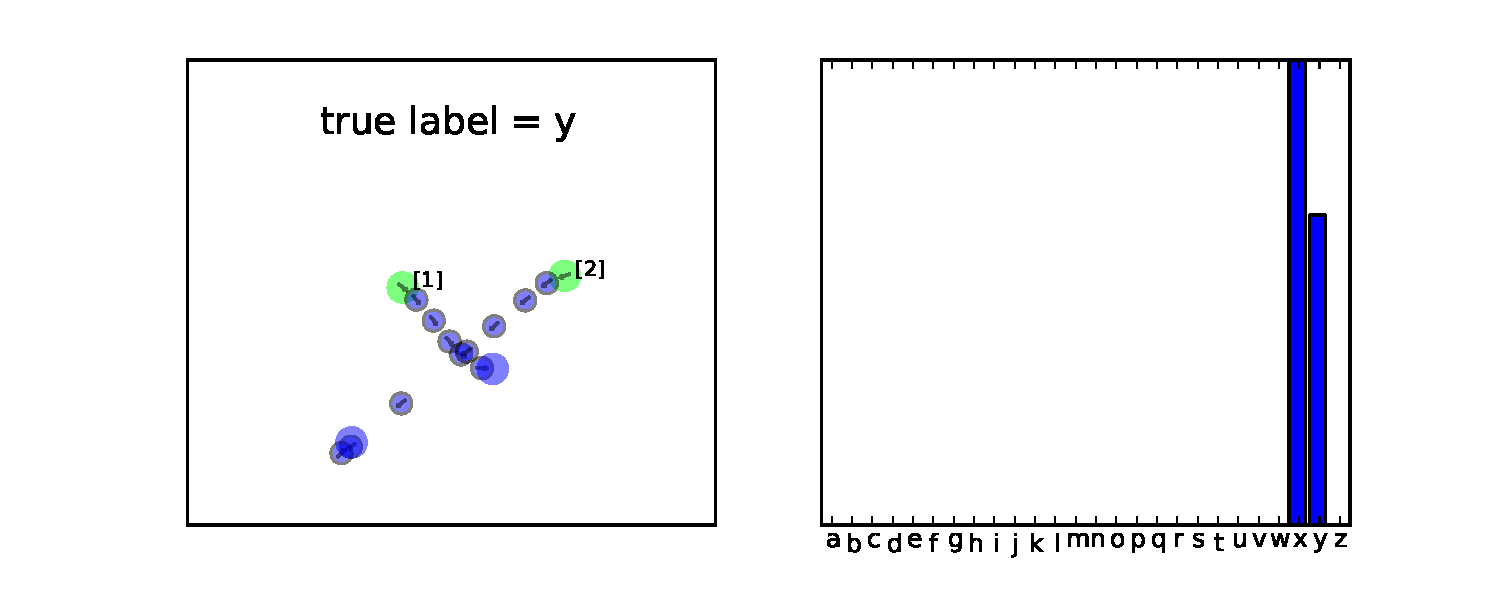
\includegraphics[width=.95\linewidth]{figures/icml-uright-interesting-134.pdf}\\
  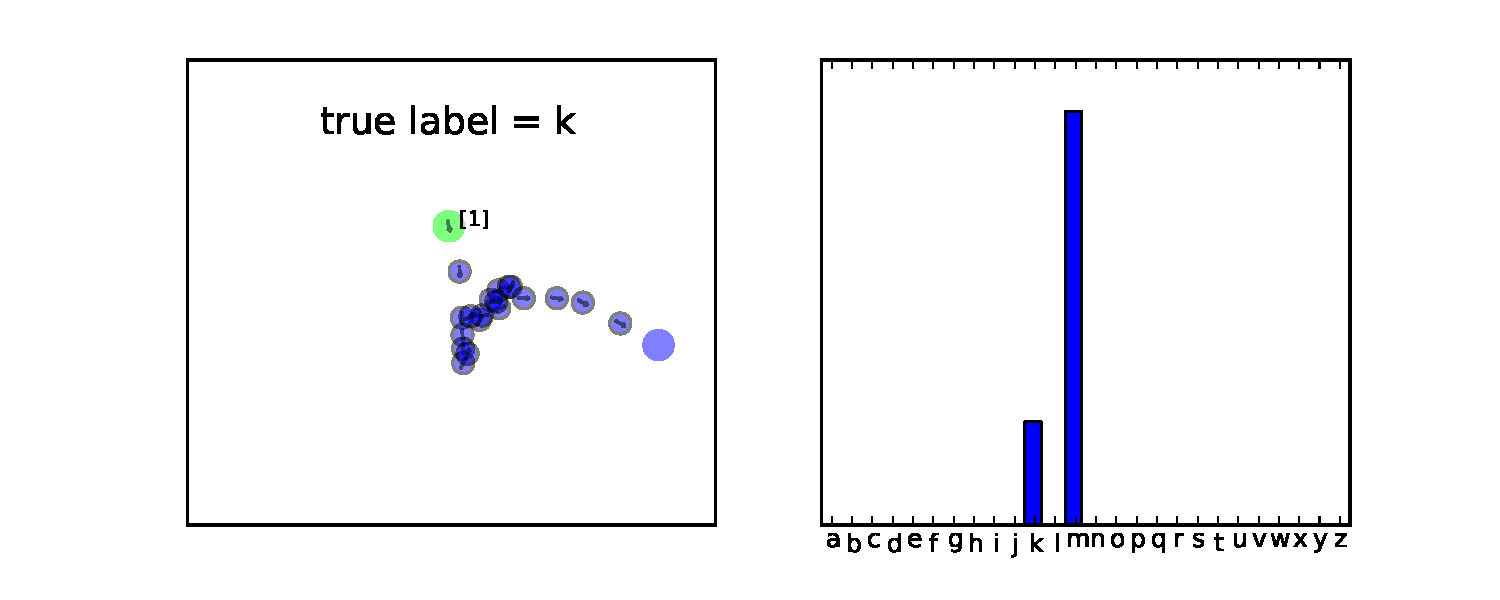
\includegraphics[width=.95\linewidth]{figures/icml-uright-interesting-70.pdf}\\
  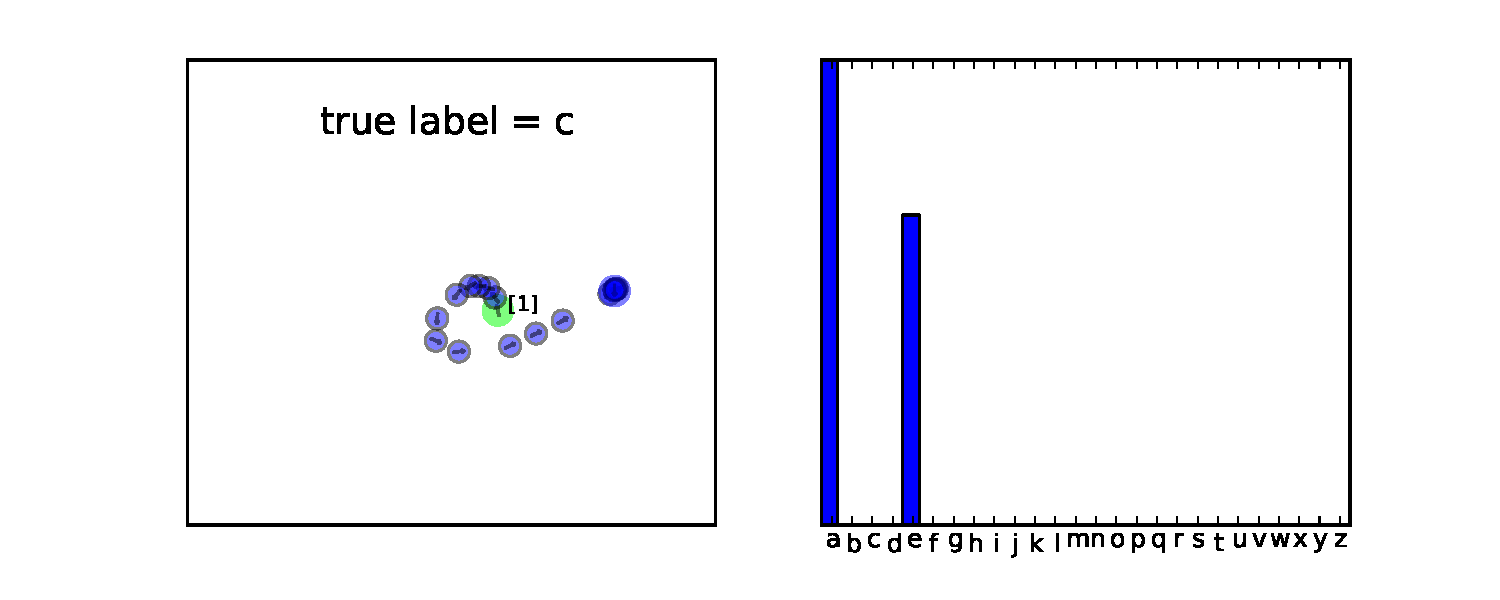
\includegraphics[width=.95\linewidth]{figures/icml-uright-interesting-248.pdf}\\
  \caption{Some examples misclassified by Majority but correctly
    classified by MinKL. Each handwriting trajectory is shown on the
    left and the corresponding empirical distribution induced by its
    $5$ neighbors is shown on the right.}
  \label{fig:uright-mistakes}
\end{center}
\vskip -0.2in
\end{figure}

\begin{figure}[hb]
\vskip 0.2in
\begin{center}
\centering
\subfigure[uRight]{
  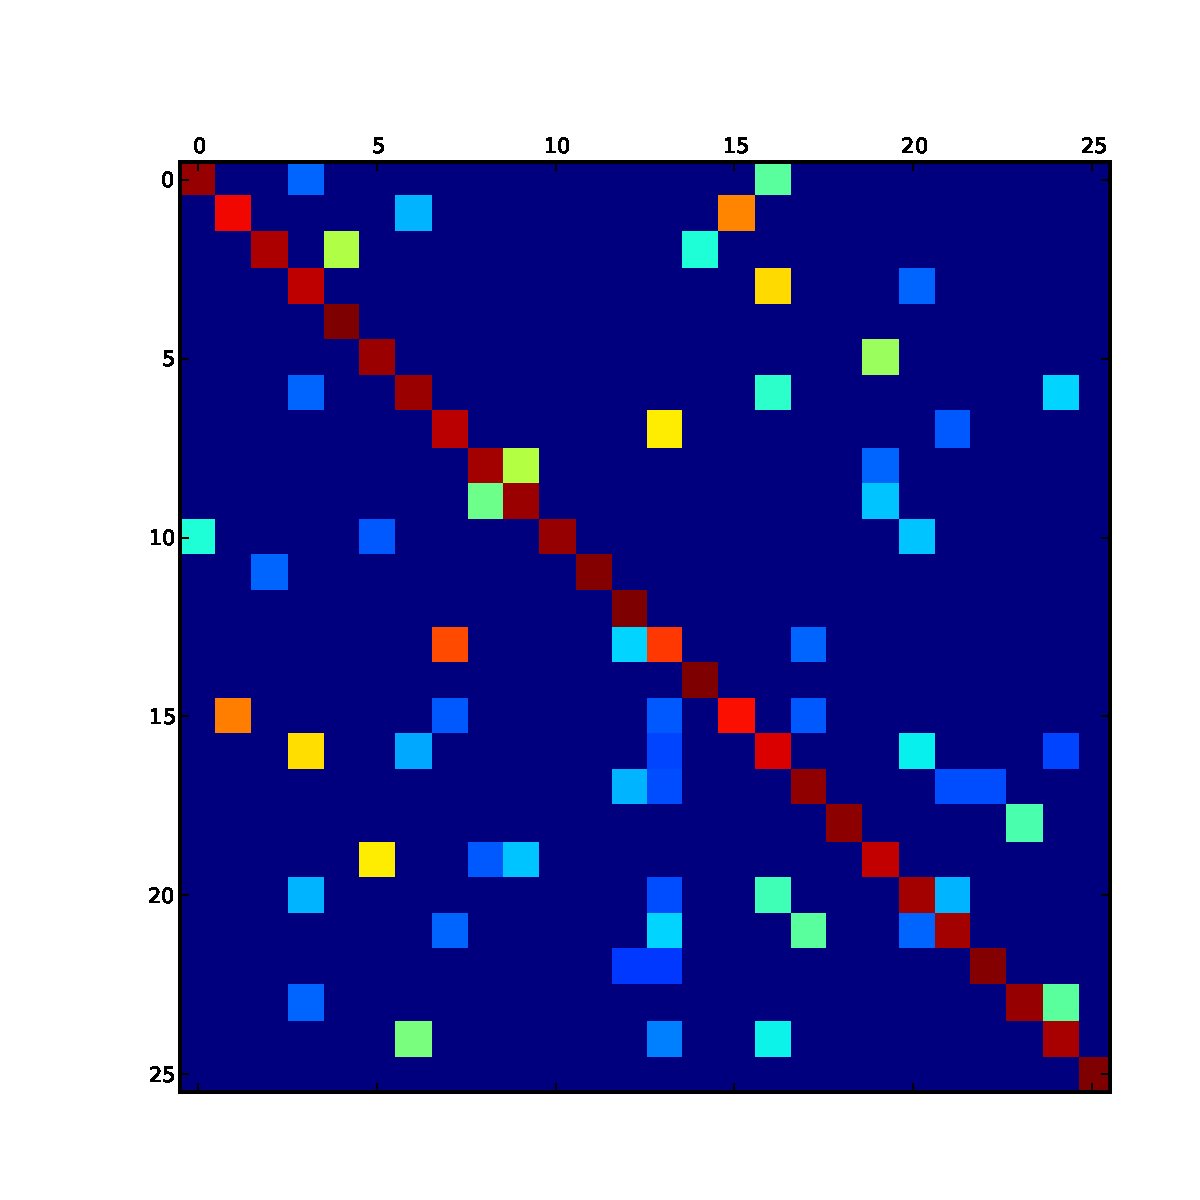
\includegraphics[width=.3\linewidth]{figures/icml-uright-matrix-82.pdf}
}
\subfigure[MNIST]{
  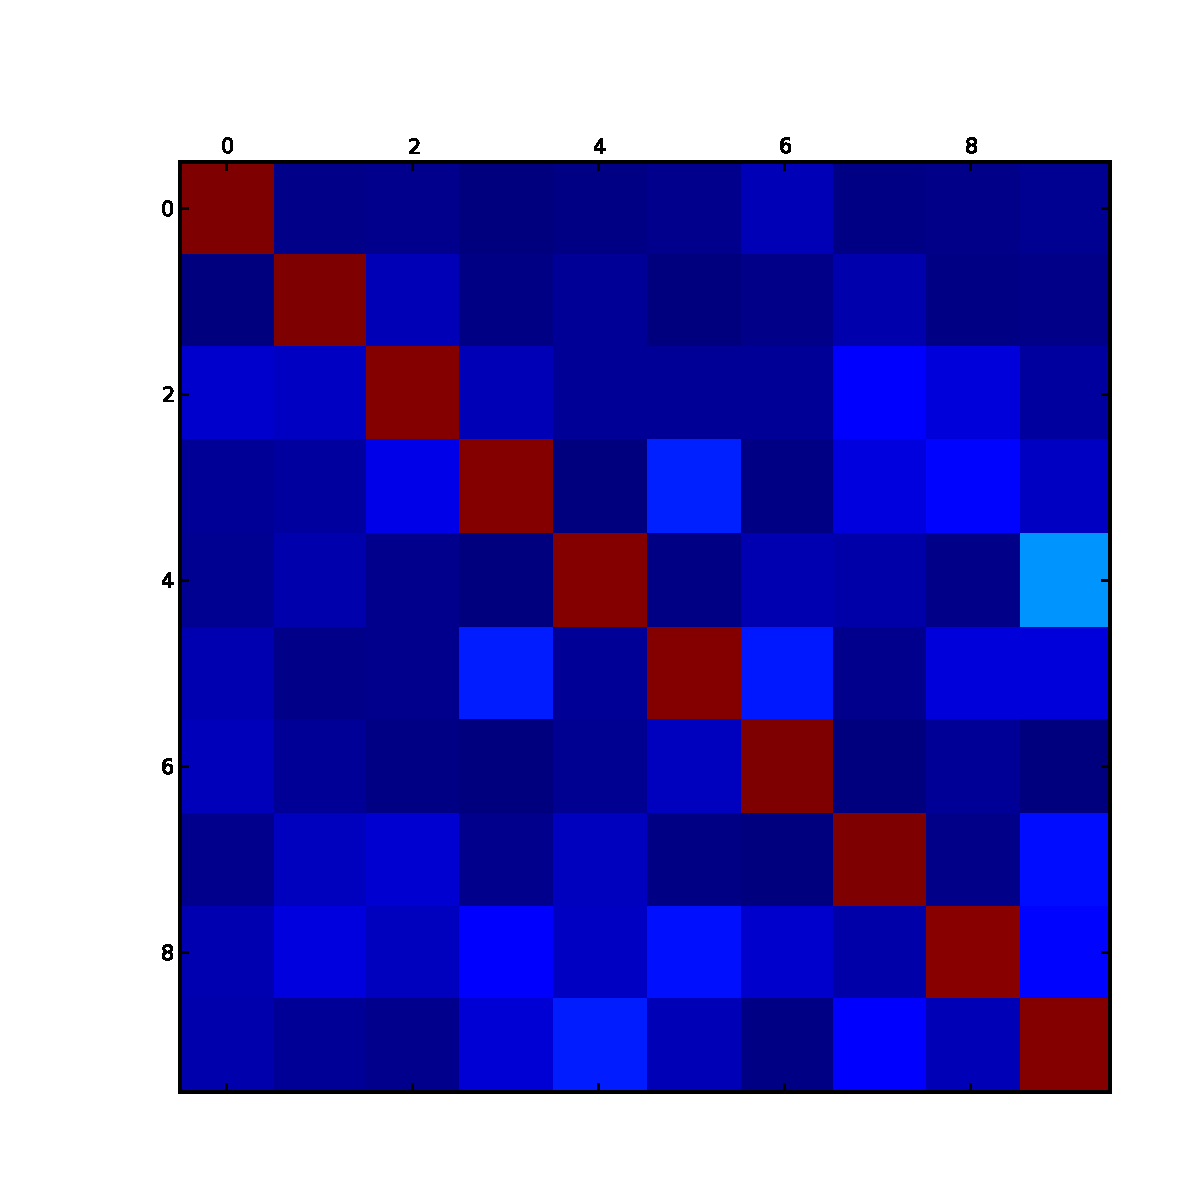
\includegraphics[width=.3\linewidth]{figures/icml-mnist-matrix.pdf}
}
\subfigure[SVHN]{
  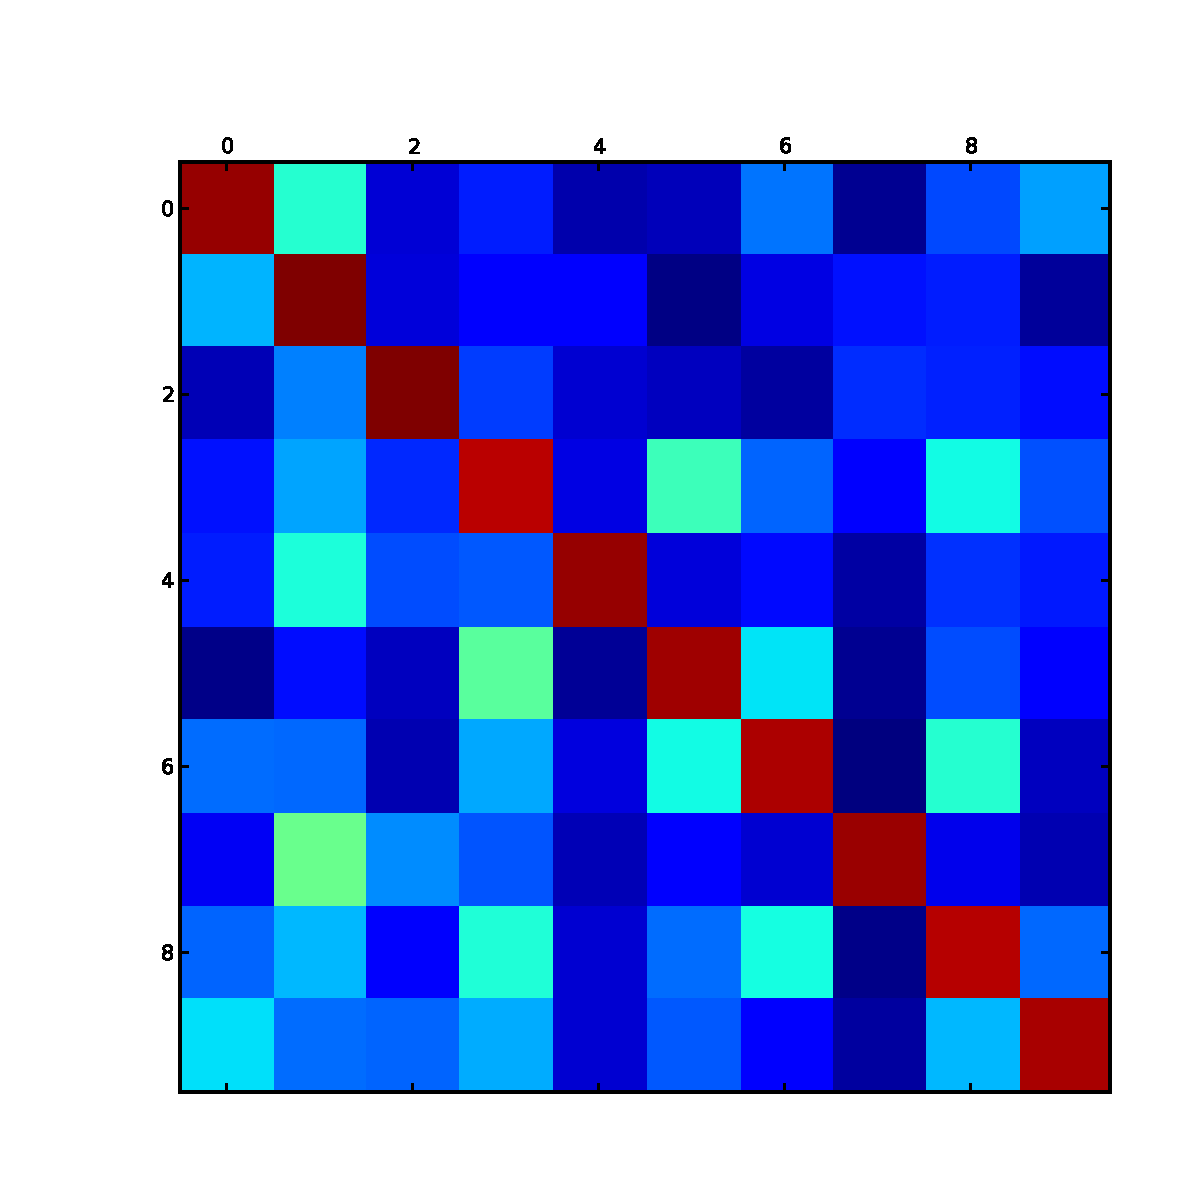
\includegraphics[width=.3\linewidth]{figures/icml-svhn-matrix.pdf}
}
\caption{A visualization of the empirical center distributions. Each row
  in each matrix corresponds to each class. }
\label{fig:matrix}
\end{center}
\vskip -0.2in
\end{figure}


\subsection{MNIST}
The MNIST dataset~\cite{Lecun1998} contains images of handwritten
digits. Each example is a 28x28 grayscale image. There are 60000
training examples and 10000 test examples included in the dataset. We
prepropressed the data by de-skewing and downsampling the images. After
the preprocessing, we ran PCA on the training data. The feature vector
of each example corresponds to the coefficients of the first 100 PCA
components. The Euclidean distance is used as the similarity measure
in the neighborhood calculation.

The test error rates we obtained from our experiment are comparable to
what reported in~\cite{Lecun1998}. The performance of both MinKL and
Majority are very similar for this dataset. The lowest error rate of 1.89\% for
Majority and 1.90\% for MinKL was obtained when $k = 5$.
Figure~\ref{fig:mnist-svhn-results} shows the test error rates of
both MinKL and Majority obtained using different $k$. 

\begin{figure}[ht]
\vskip 0.2in
\begin{center}
\centering
\subfigure[MNIST]{
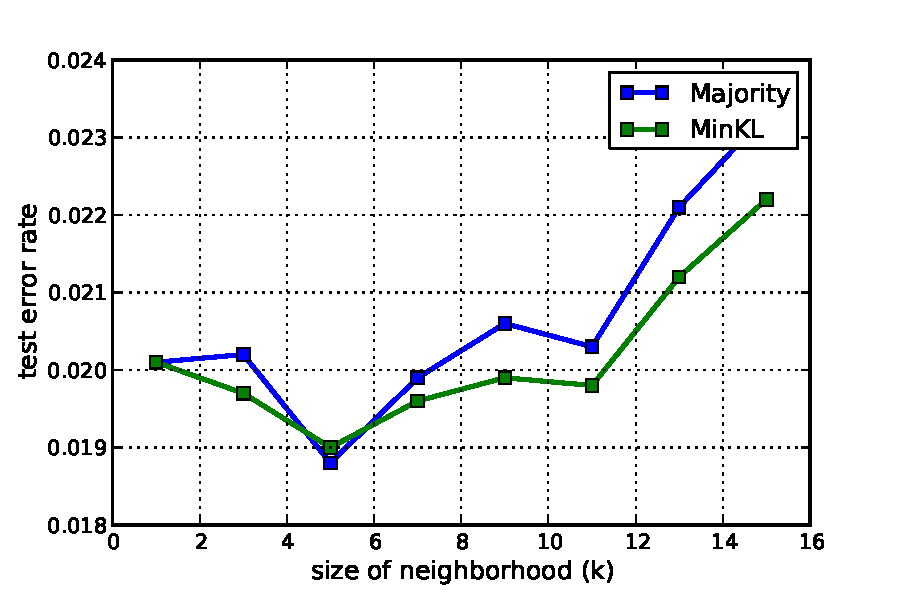
\includegraphics[width=.95\linewidth]{figures/icml-mnist-error.pdf}
}\\
\subfigure[SVHN]{
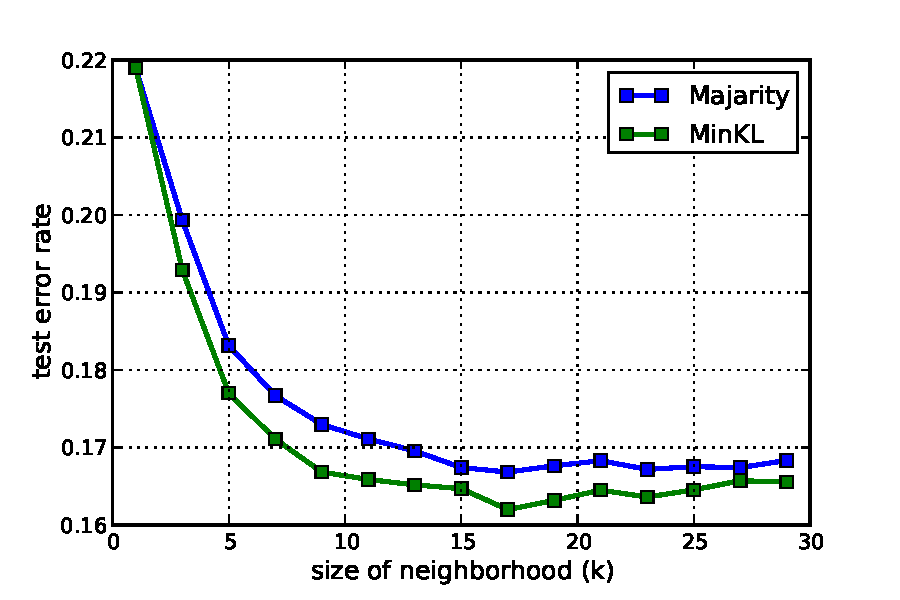
\includegraphics[width=.95\linewidth]{figures/icml-svhn-error.pdf}
}
\caption{MNIST and SVHN results}
\label{fig:mnist-svhn-results}
\end{center}
\vskip -0.2in
\end{figure}


\subsection{SVHN}
The SVHN dataset~\cite{Netzer2011} contains images of digits taken
from the Google street view data. It is considered a harder dataset
than MNIST due a higher degree of variations. Each example in SVHN is
a 32x32 RGB image. There are 73257 training examples and 26032 test
examples included in the dataset. We computed, for each example, the
HOG features~\cite{Dalal2005} using the block size of 4x4 with 8
orientations per block. The Manhattan distance is used as the
similarity measure in the neighborhood calculation.

In~\cite{Netzer2011}, the test error rate for HOG features combined
with an SVM is reported to be around 15\%. In our experiment, the test
error rates of both MinKL and Majority are between 16\% to 17\% with
MinKL performing slightly better than Majority at every $k >
1$. Figure~\ref{fig:mnist-svhn-results} shows the test error rates of
both MinKL and Majority obtained using different $k$.

\section{Discussion}
\label{sec:discussion}

In our experiments with \textbf{SYN-1} and \textbf{SYN-2}, we observed
that MinKL performs significantly better than Majority when $n$ is
small. This result also confirms our intuition we have on the toy
example in Figure~\ref{fig:toy_example}. Our explanation for this
boost in performance is the fact that, for small $n$ (implied a small
$k$), the majority rule is prone to error because the prediction is
based on solely the majority of the empirical class distribution
$\Pemp$ induced from a relatively small $k$; while the MinKL
rule makes the prediction based on the entire class distribution.

From our analysis in Section~\ref{sec:min_kl}, we show that our
approach will perform optimally when the training set has $\delta_k =
0$. However, when $\delta_k$ is small relative to the distance between
the center distributions of different classes, we expect our approach
to perform reasonably well. In \textbf{SYN-3}, we deliberately
designed the dataset such that its $\delta_k$ is quite large. As
expected, the error rates for our approach are inferior to those of
the majority rule even when $n$ is small.


% why Syn-3 fail
In a sense, our approach naturally incoporates the infomation from the
label space into the classification. The label space information is
encoded in the form of the center distribution $\Qemp$. The
performance of our approach depends on how well the center
distribution $\Qemp$ can model the examples of the
class.


neighborhood distributions of different classes are. 


If the
prototypical distributions are similar to each other, then our
approach will not perform well. A workaround is to maintain multiple
prototypical distributions per class.




As $n$ increases, the performance gap between the two rules decreases and
the error rate of both rules converge to the Bayes error.




We suspect that our approach will be more beneficial to problems with
a large number of classes and the confusions between classes are
non-uniform.

Our approach does not have a consistency gaurantee. It is
possible that our approach will be sub-optimal when the number of
training examples goes to infinity because the prototypical
distribution model is incorrect or insufficent. We do not worry
about this problem that much since we see our approach being used
in a small sample scenario.

In practice, other divergences might work better than the
KL-divergence. The KL-divergence is considered a special case of a
more general divergence function called
Alpha-divergence~\cite{Cichocki2010}, which is given by
\[
D^{(\alpha)}_A (p||q) = \frac{1}{\alpha(\alpha - 1)}\left( \sum_1^n
  p^{\alpha}_i q^{1-\alpha}_i - 1\right), \; \alpha \in \mathrm{R} \ \{0,1\}
\]
The KL-divergence can be expressed as $D_{KL} (p || q) = \lim_{\alpha
  \rightarrow 1} D^{(\alpha)}_A (p || q)$.  For the uRight dataset, we
were able to obtain even lower error rate by using Alpha-divergence
with $\alpha = 2$.

Our approach can be applied to other classification algorithms as
well. The $k$-NN algorithm is very computational expensive in
classifying a new example. In some applications, it is important to be
able to classify new examples quickly. A simple modification to the
$k$-NN algorithm that significanly reduces the classication time is to
keep only a small number of representatives per class and discard the
rest of the examples. This algorithm is called the $k$
nearest-centroid algorithm ($k$-NC) where only the $k$-centroids are
kept as the class representatives. In the $k$-NC, the class
distribution $\mathbf{P}_x$ can be estimating by
\[
\mathbf{P}_x(j) = \frac{e^{d(x,C(j))}}{\sum_i e^{d(x, C(i))} }
\]
We can apply MinKL to the class posterior computed this way. 


\section{Conclusions}
\label{sec:conclusion}

We suggest a simple modification to the $k$-NN algorithm.

\bibliography{library}
\bibliographystyle{icml2014}

\end{document} 


% This document was modified from the file originally made available by
% Pat Langley and Andrea Danyluk for ICML-2K. This version was
% created by Lise Getoor and Tobias Scheffer, it was slightly modified  
% from the 2010 version by Thorsten Joachims & Johannes Fuernkranz, 
% slightly modified from the 2009 version by Kiri Wagstaff and 
% Sam Roweis's 2008 version, which is slightly modified from 
% Prasad Tadepalli's 2007 version which is a lightly 
% changed version of the previous year's version by Andrew Moore, 
% which was in turn edited from those of Kristian Kersting and 
% Codrina Lauth. Alex Smola contributed to the algorithmic style files.  
